% interactcadsample.tex
% v1.03 - April 2017

\documentclass[]{interact}

\usepackage{epstopdf}% To incorporate .eps illustrations using PDFLaTeX, etc.
\usepackage{subfigure}% Support for small, `sub' figures and tables
%\usepackage[nolists,tablesfirst]{endfloat}% To `separate' figures and tables from text if required

\usepackage{natbib}% Citation support using natbib.sty
\bibpunct[, ]{(}{)}{;}{a}{}{,}% Citation support using natbib.sty
\renewcommand\bibfont{\fontsize{10}{12}\selectfont}% Bibliography support using natbib.sty

\theoremstyle{plain}% Theorem-like structures provided by amsthm.sty
\newtheorem{theorem}{Theorem}[section]
\newtheorem{lemma}[theorem]{Lemma}
\newtheorem{corollary}[theorem]{Corollary}
\newtheorem{proposition}[theorem]{Proposition}

\theoremstyle{definition}
\newtheorem{definition}[theorem]{Definition}
\newtheorem{example}[theorem]{Example}

\theoremstyle{remark}
\newtheorem{remark}{Remark}
\newtheorem{notation}{Notation}

% see https://stackoverflow.com/a/47122900

% Pandoc citation processing

\usepackage{hyperref}
\usepackage[utf8]{inputenc}
\def\tightlist{}


\begin{document}

\articletype{ARTICLE TEMPLATE}

\title{Why shouldn't you use numerical tests to diagnose the linear
regression models?}


\author{\name{Weihao Li$^{a}$, Dianne Cook$^{a}$, Emi Tanaka$^{a}$}
\affil{$^{a}$Department of Econometrics and Business Statistics, Monash
University, Clayton, VIC, Australia}
}

\thanks{CONTACT Weihao
Li. Email: \href{mailto:weihao.li@monash.edu}{\nolinkurl{weihao.li@monash.edu}}, Dianne
Cook. Email: \href{mailto:dicook@monash.edu}{\nolinkurl{dicook@monash.edu}}, Emi
Tanaka. Email: \href{mailto:emi.tanaka@monash.edu}{\nolinkurl{emi.tanaka@monash.edu}}}

\maketitle

\begin{abstract}
Abstract to fill.
\end{abstract}

\begin{keywords}
visual inference; model diagnostics;
\end{keywords}

problem: residual plot diagnostics conventional test: too sensitive

background:

\begin{enumerate}
\def\labelenumi{\arabic{enumi}.}
\tightlist
\item
  residual plot for model diagnostics
\end{enumerate}

\begin{enumerate}
\def\labelenumi{\alph{enumi}.}
\tightlist
\item
  residual is widely used
\item
  what are the types of residual plots
\item
  comparison
\end{enumerate}

\begin{enumerate}
\def\labelenumi{\arabic{enumi}.}
\setcounter{enumi}{1}
\tightlist
\item
  conventional test: F, BP
\item
  visual test: lineup, theory
\end{enumerate}

desc of experiment: 1. simulation setup 2. experimental design 3. result

comparison of conventional tests: 1. power (visual test vs.~conventional
test) (visual test most different one (everything test, any departure))
plot figure in a paper, desc, exp 2. investigate the difference (gap),
give examples 3. conventional is too sensitive 4. make conventional less
sensitive (vary alpha)

conclusion: 1. too sensitive, visual test is needed/preferable 2. visual
test is infeasible in large scale (expensive) 3. future work (role of
computer vision)

\hypertarget{introduction}{%
\section{Introduction}\label{introduction}}

Regression diagnostics conventionally involve evaluating the fitness of
the proposed model, detecting the presence of influential observations
and outliers, checking the validity of model assumptions and many more.
Common diagnostic techniques including summary statistics, hypothesis
testing, and data plots are essential tools for a systematic and
detailed examination of the regression model
\citep{mansfield1987diagnostic}.

\hypertarget{diagnostic-plots}{%
\subsection{Diagnostic plots}\label{diagnostic-plots}}

Regression analysis is a field of study with at least a hundred years of
history. Many of those regression diagnostic methods and procedures are
mature and well-established in books first published in the twentieth
century, such as \citet{draper_applied_2014},
\citet{montgomery_introduction_2012}, \citet{belsley_regression_1980},
\citet{cook_applied_1999} and \citet{cook1982residuals}. Regardless of
the level of difficulty of the book, one will find the importance and
usefulness of diagnostic plots being emphasized again and again.
Checking diagnostic plots is also the recommended starting point for
validating model assumptions like normality, homoscedasticity and
linearity \citep{anscombe_examination_1963}.

Graphical summaries in which residuals are plotted against fitted values
or other functions of the predictor variables that are approximately
orthogonal to residuals are refereed to as standard residual plots. They
are commonly used to identify patterns which are indicative of
nonconstant error variance or non-linearity \citep{cook1982residuals}.
Raw residuals and studentized residuals are the two most frequently used
residuals in standard residual plots. The debt on which type of
residuals should be used always present. While raw residuals are the
most common output of computer regression software package, by applying
a scaling factor, the ability of revealing nonconstant error variance in
standard residual plots will often be enhanced by studentized residuals
in small sample size \citep{gunst2018regression}.

As a two-dimensional representation of a model in a \(p\)-dimensional
space, standard residual plots project data points onto the variable of
the horizontal axis, which is a vector in \(p\)-dimensional space.
Observations with the same projection will be treated as equivalent as
they have the same position of the abscissa. Therefore, standard
residual plots are often useful in revealing model inadequacies in the
direction of the variable of the horizontal axis, but could be
inadequate for detecting patterns in other directions, especially in
those perpendicular to the variable of the horizontal axis. Hence, in
practice, multiple standard residual plots with different horizontal
axes will be examined.

Overlapping data points is a general issue in scatter plots not limited
to standard residual plots, which often makes plots difficult to
interpret because visual patterns are concealed. Thus, for relatively
large sample size, \citet{cleveland1975graphical} suggests the use of
robust moving statistics as reference lines to give aids to eye in
seeing patterns, which nowadays, are usually replaced with a spline or
local polynomial regression line.

Other types of data plots that are often used in regression diagnostics
include partial residual plots and probability plots. Partial residual
plots are useful supplements to standard residual plots as they provide
additional information on the extent of the non-linearity. Probability
plots can be used to compare the sampling distribution of the residuals
to the normal distribution for assessing the normality assumptions.

\hypertarget{hypothesis-testing}{%
\subsection{Hypothesis testing}\label{hypothesis-testing}}

In addition to diagnostic plots, researcher may also perform formal
tests for detecting model defects. Depends on the alternative, variety
of tests can be applied. For example, for testing heteroskedasticity,
one may use the White test
\citep{white_heteroskedasticity-consistent_1980} or the Breusch-Pagan
test \citep{breusch_simple_1979}. And for testing non-linearity, there
are RESET test \citep{ramsey_tests_1969} and F-test.

As discussed in \citet{cook1982residuals}, most residual based tests for
a particular type of departures from model assumptions are sensitive to
other types of departures. Especially, outliers will often incorrectly
trigger the rejection of null hypothesis despite the residuals are
well-behaved \citep{cook_applied_1999}. This can be largely avoided in
diagnostic plots as experienced analysts can evaluate the acceptability
of assumptions flexibly, even in the presence of outliers. Furthermore,
\citet{montgomery_introduction_2012} stated that based on their
experience, statistical tests are not widely used in regression
diagnostics. Most importantly, the same or even larger amount of
information can be provided by diagnostic plots than the corresponding
tests in most empirical studies. But still, the effectiveness of
statistical tests shall not be disrespected. Statistical tests have
chance to provide analysts with unique information. There are also
situations where no suitable diagnostic plots can be found for a
particular violation of the assumptions, or excessive diagnostic plots
need to be checked. One will have no choice but to rely on statistical
tests if there is any. A good regression diagnostic practice should be a
combination of both methods.

\hypertarget{visual-inference}{%
\subsection{Visual inference}\label{visual-inference}}

Diagnostic plots are

\hypertarget{experimental-design}{%
\section{Experimental design}\label{experimental-design}}

\hypertarget{data-processing}{%
\section{Data processing}\label{data-processing}}

\hypertarget{results}{%
\section{Results}\label{results}}

\hypertarget{overview-of-the-data}{%
\subsection{Overview of the Data}\label{overview-of-the-data}}

We collected 400 lineup evaluations made by 20 participants in
experiment I and 880 lineup evaluations made by 44 participants in
experiment II. In total, 442 unique lineups were evaluated by 64
subjects. In experiment I, one of the participants skipped all 20
lineups. Hence, the submission was rejected and removed from the
dataset. In experiment II, there was a participant failed one of the two
attention checks, but there was no further evidence of low-effort
throughout the experiment. Therefore, the submission was kept.

\hypertarget{power-comparision}{%
\subsection{Power comparision}\label{power-comparision}}

\begin{enumerate}
\def\labelenumi{\arabic{enumi}.}
\tightlist
\item
  power (visual test vs.~conventional test) (visual test most different
  one (everything test, any departure)) plot figure in a paper, desc,
  exp
\item
  investigate the difference (gap), give examples
\item
  conventional is too sensitive
\item
  make conventional less sensitive (vary alpha)
\end{enumerate}

To model the power of visual test, 10 logistic regression were fit for
different number of evaluations ranged from one to five and two
different types of simulation setting. All 10 models used natural
logarithm of the effect size as the only fixed effect, and whether the
test successfully rejects the null hypothesis as the response variable.
Given the way we define the effect size, it was expected that with
larger effect size, both conventional test and visual test will have
higher probability in rejecting the null hypothesis when it is not true.
The modelling result summarized in \ref{tab:powerglmcubic} and
\ref{tab:powerglmheter} aligned with the expectation as the coefficients
of natural logarithm of the effect size are positive and significant
across all 10 models.

Figure \ref{fig:power-com} illustrates the fitted models, while
providing the local constant estimate of the power of F-test and
Breusch--Pagan test for comparison. Data for the conventional test is
simulated under the model setting described in section \ldots{} and
5000000 samples are drawn for both cubic and heteroskedasticity model.
From Figure \ref{fig:power-com}, it can be observed that the fitted
power of visual test increased as the number of evaluations increased
for both cubic and heteroskedasticity model.

For heteroskedasticity model, this phenomenon was more obvious as the
power of visual tests with evaluations greater than two were always
greater than those with evaluations smaller than two.

For cubic model, the separation between curves was small. The estimated
power of visual tests with three to five evaluations were almost
identical to each other in regards of effect size. In addition, all five
curves peaked at one as effect size increased, suggesting that
identification of non-linearity as a visual task can be completed
reliably by human as long as the departure from null hypothesis is large
enough.

As shown in Figure \ref{fig:power-com}, both F-test and Breusch--Pagan
test generally possessed greater power than visual test. A visual tests
is a collection of test against any alternatives that would create
visual discoverable features, while a conventional test is usually
targeting at a pre-specified alternative. Considering the data
generating process of the model defect was known and controlled in this
research, where all other alternatives have been eliminated except the
one we concerned, the result was suggested that conventional tests were
more sensitive to violations of linearity and homoscedasticity
assumption than visual tests.

It was also found that there was a noticeable gap between curves of the
conventional test and the visual test at around
\(log(\text{effect size}) = 0\) for the cubic model and
\(log(\text{effect size}) = 2.5\) for the heteroskedasticity model,
where the differences in power were greater than 0.6. We further
analysed the lineups with correspoding effect sizes. Figure
\ref{fig:cubic-hard} and \ref{fig:heter-hard} showed that human was
indeed hard to identify the patterns at this level of difficulty. The
visual difference between the true data plot and null plots were almost
unnoticeable.

\hypertarget{effect-of-parameters-on-power-of-the-visual-test}{%
\subsection{Effect of parameters on power of the visual
test}\label{effect-of-parameters-on-power-of-the-visual-test}}

The previous section focuses on the change of effect size relative to
the power of the visual test. However, effect size is only a one
dimensional summarisation of parameters used in data simulation.
Individual factor embedded in the simulation process should also be
analysed.

In cubic model, two major factors that influencing the strength of the
signal are \(a\) and \(b\). Figure \ref{fig:power-com-cubic-a} and
\ref{fig:power-com-cubic-a} illustrates 30 different logistic
regressions fit for different number of evaluations and different number
of observations \(n\). The regressor used in these models was
\(|a|/\sigma\) since the noise level \(\sigma\) needed to be taken into
account. From the figures, we can observe \ldots{}

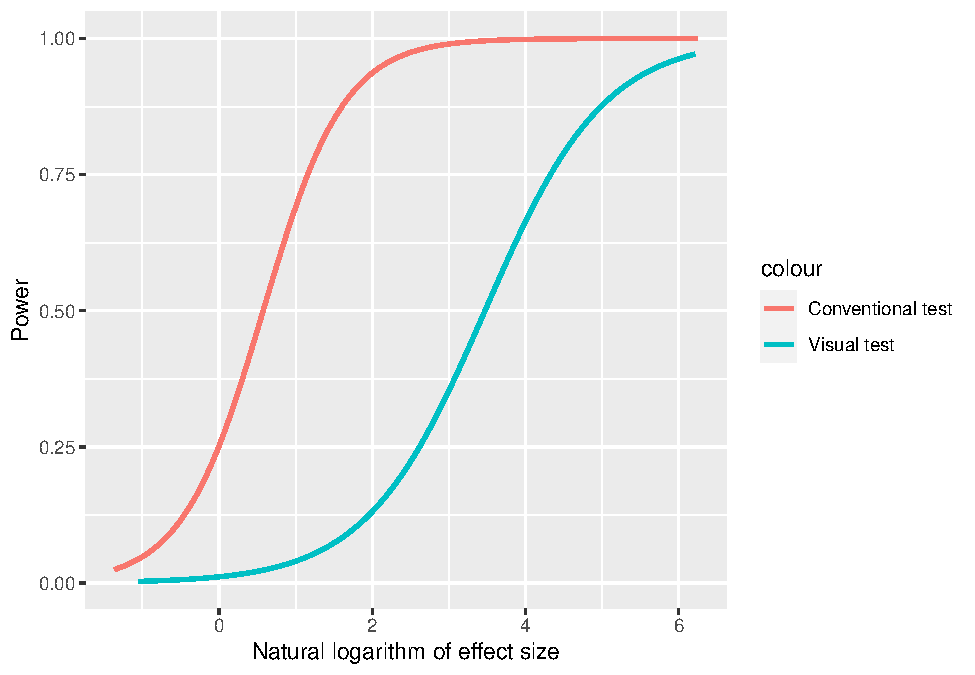
\includegraphics{paper_comparison_files/figure-latex/power-vs-log-effect-size-1.pdf}

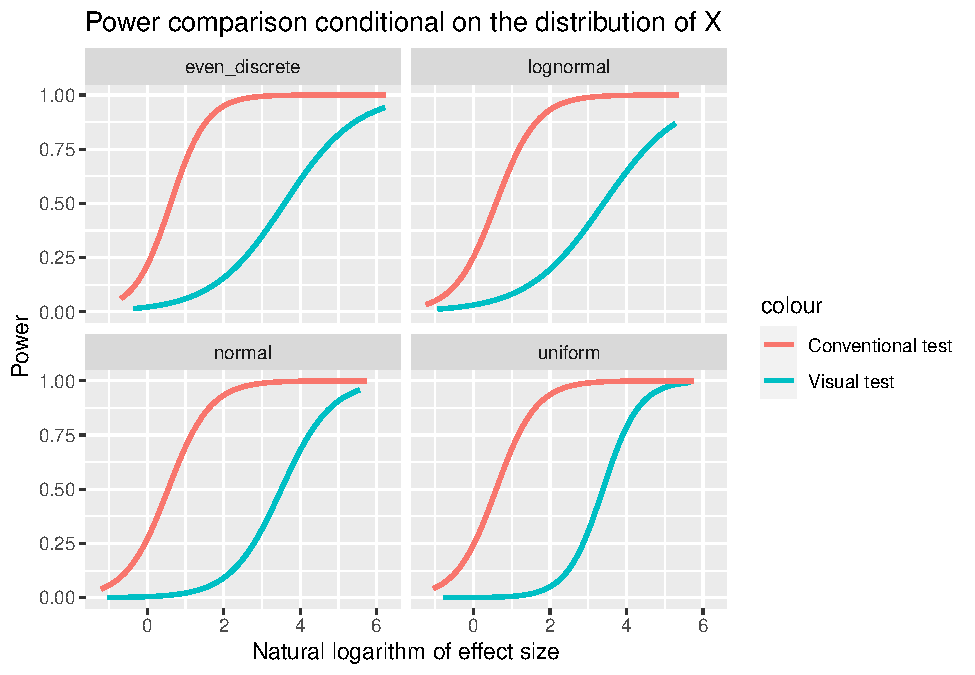
\includegraphics{paper_comparison_files/figure-latex/power-vs-log-effect-size-given-x-dist-1.pdf}

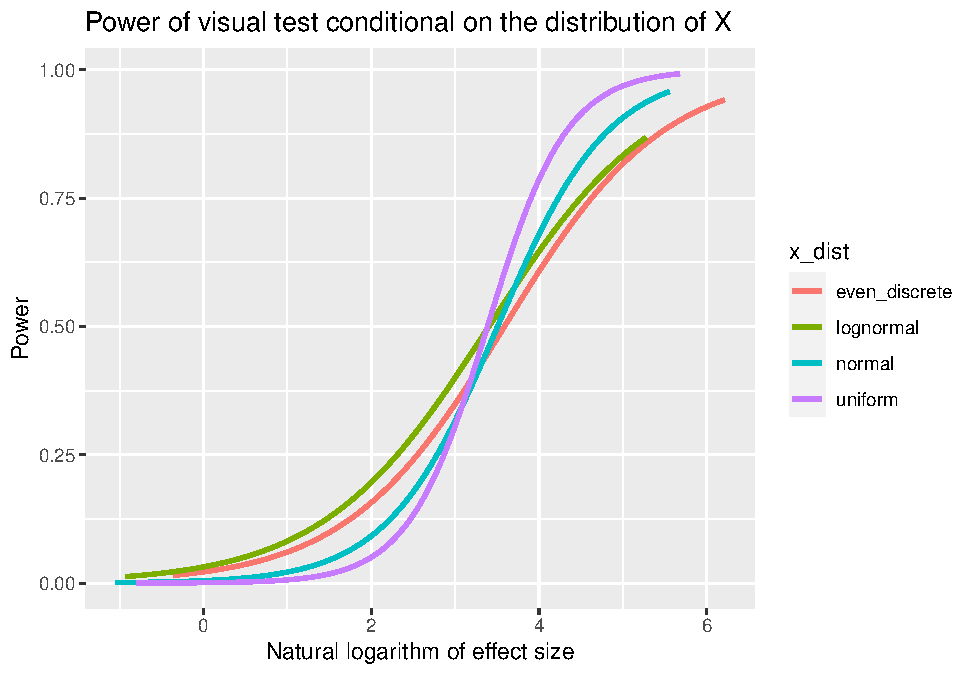
\includegraphics{paper_comparison_files/figure-latex/power-of-visual-test-given-x-dist-1.pdf}

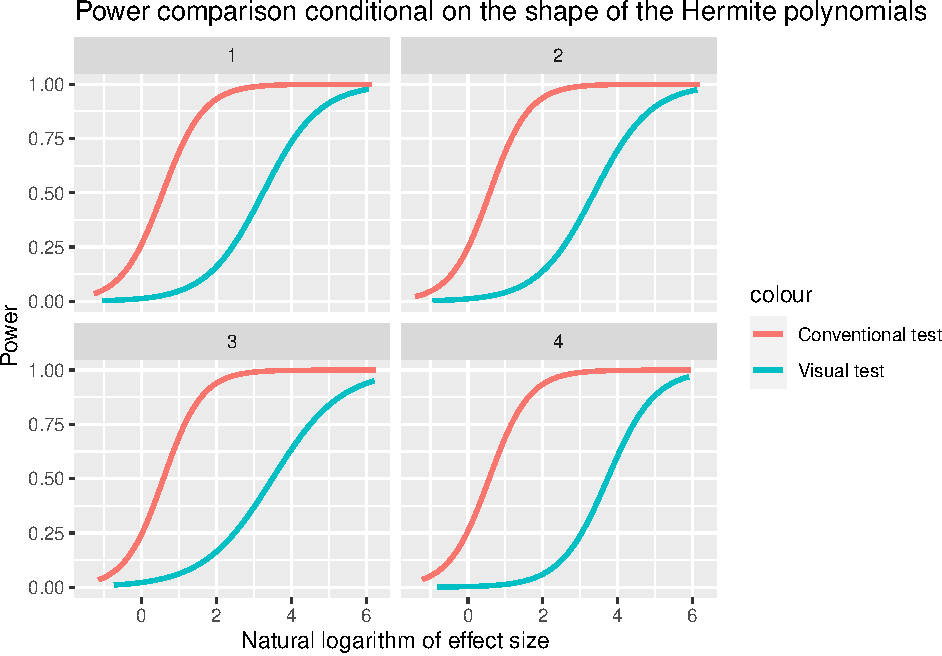
\includegraphics{paper_comparison_files/figure-latex/power-vs-log-effect-size-given-shape-1.pdf}

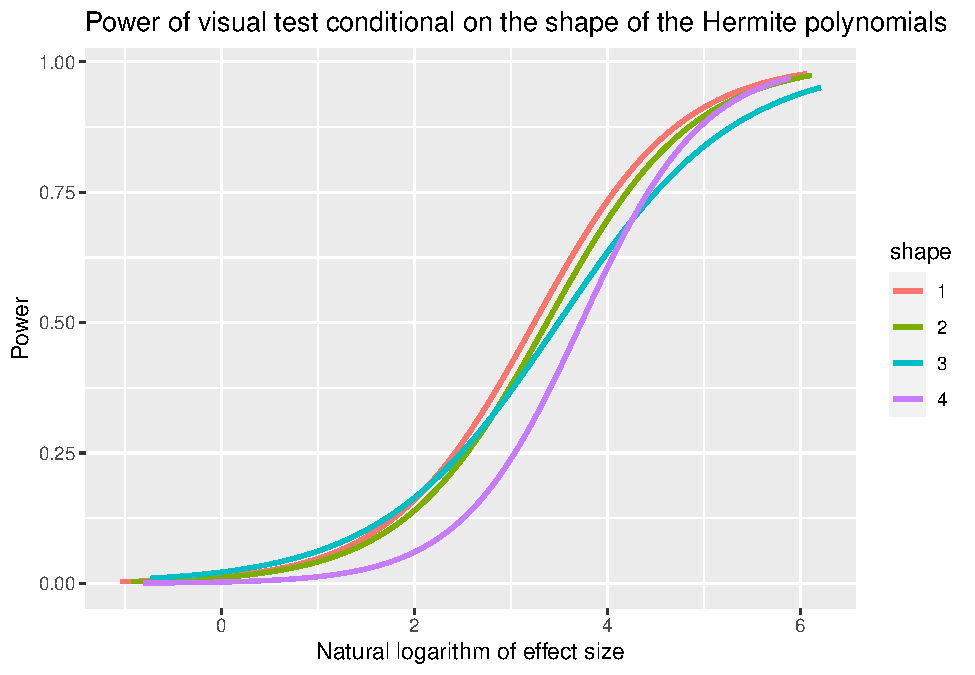
\includegraphics{paper_comparison_files/figure-latex/power-of-visual-test-given-shape-1.pdf}

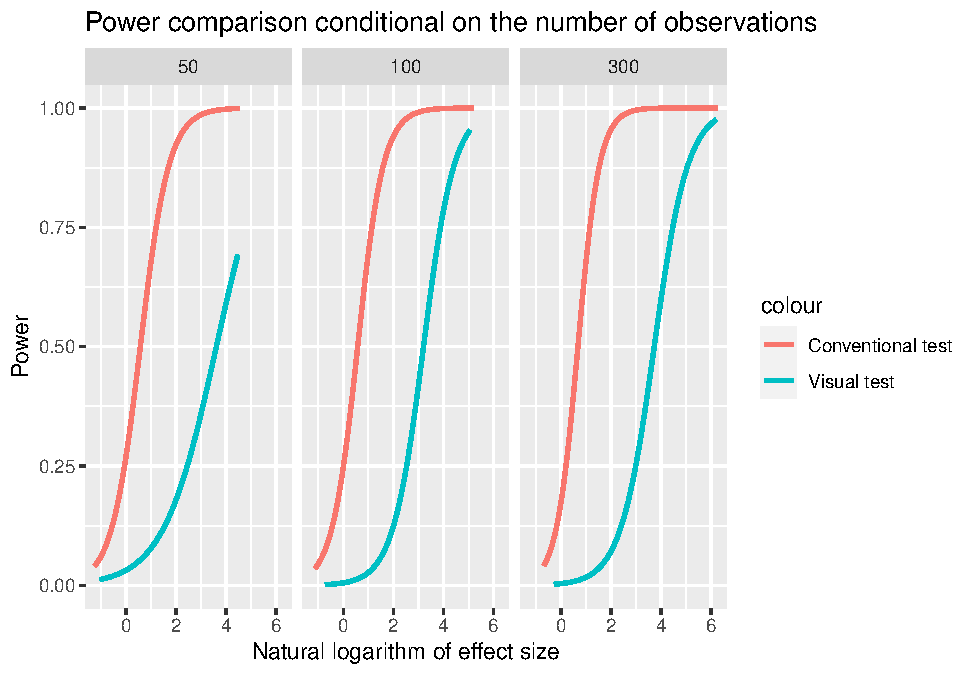
\includegraphics{paper_comparison_files/figure-latex/power-vs-log-effect-size-given-number-of-observations-1.pdf}

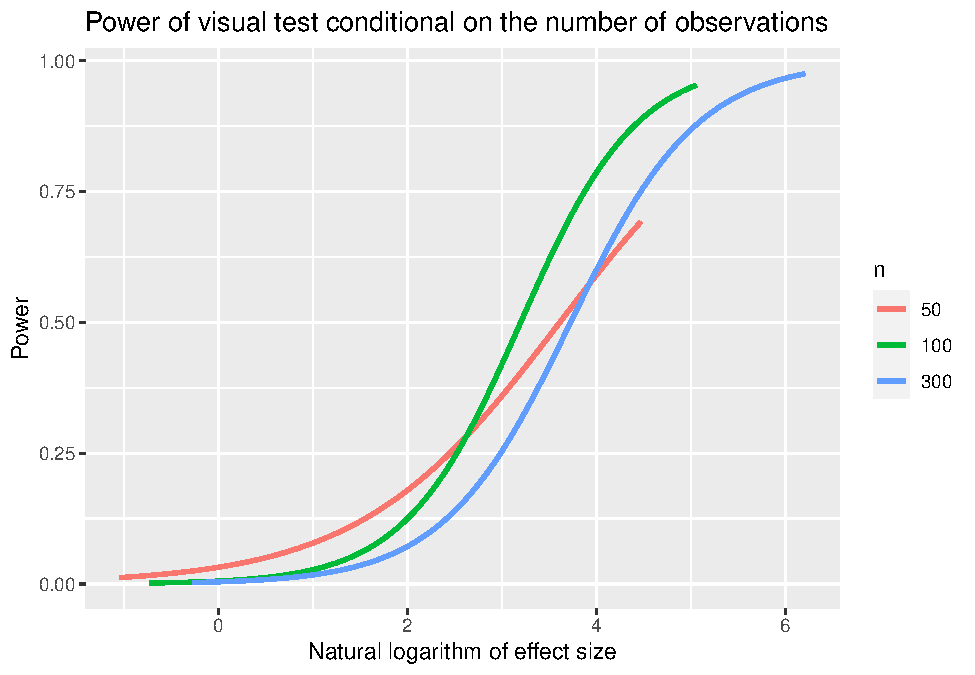
\includegraphics{paper_comparison_files/figure-latex/power-of-visual-test-given-number-of-observations-1.pdf}

\bibliographystyle{tfcad}
\bibliography{paper.bib}




\end{document}
